% Pipeline Diagram: Raw Signal → Pulse → Scalogram → Few-Shot Classification
% VERTICAL LAYOUT - Original style preserved
% Compile: pdflatex pipeline.tex

\documentclass[border=20pt]{standalone}
\usepackage[utf8]{inputenc}
\usepackage{tikz}
\usetikzlibrary{shapes.geometric, arrows.meta, positioning, shadows, calc, fit, backgrounds}

% Define colors (ORIGINAL)
\definecolor{rawcolor}{RGB}{52, 152, 219}      % Blue
\definecolor{pulsecolor}{RGB}{46, 204, 113}    % Green  
\definecolor{scalocolor}{RGB}{155, 89, 182}    % Purple
\definecolor{fewshotcolor}{RGB}{231, 76, 60}   % Red
\definecolor{arrowcolor}{RGB}{44, 62, 80}      % Dark gray
\definecolor{bglight}{RGB}{245, 245, 245}      % Light background

\begin{document}

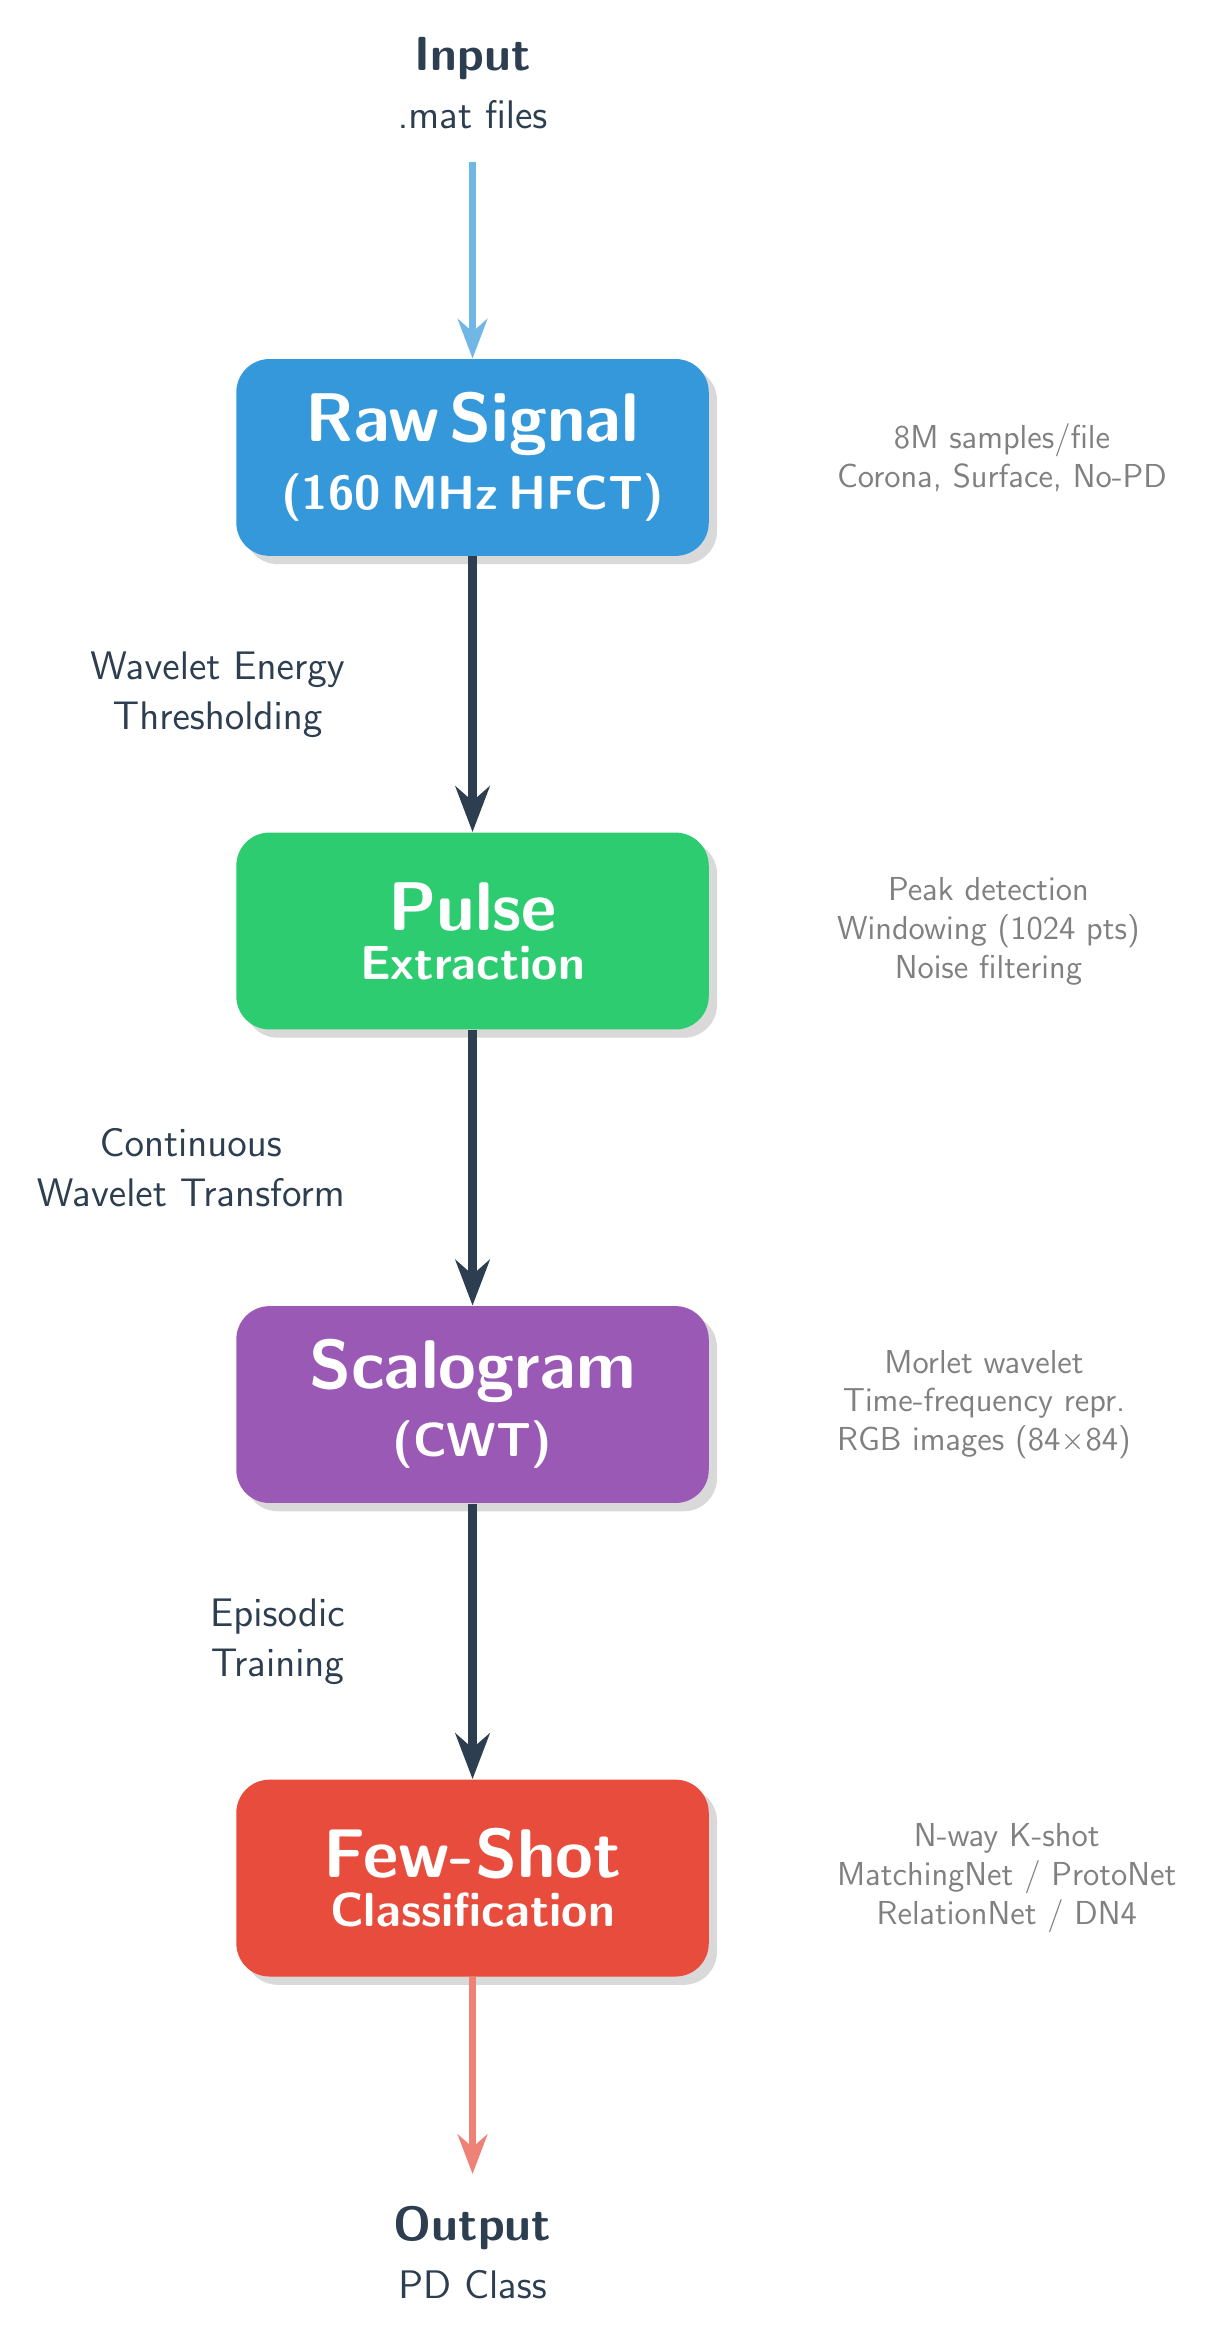
\begin{tikzpicture}[
    % Node styles - ORIGINAL STYLE
    block/.style={
        rectangle, 
        rounded corners=12pt,
        minimum width=6cm, 
        minimum height=2.5cm,
        text centered, 
        text width=5.5cm,
        font=\sffamily\bfseries,
        draw=none,
        drop shadow={shadow xshift=3pt, shadow yshift=-3pt, opacity=0.3}
    },
    % Arrow style - THICKER
    arrow/.style={
        ->,
        >=Stealth,
        line width=3pt,
        color=arrowcolor
    },
    % Label style - LARGER FONT
    label/.style={
        font=\sffamily\Large,
        text=arrowcolor,
        align=center
    },
    % Sub-description style - LARGER FONT
    subdesc/.style={
        font=\sffamily\large,
        text=gray,
        align=center
    }
]

% ===== MAIN PIPELINE BLOCKS (VERTICAL) =====

% Block 1: Raw Signal (TOP)
\node[block, fill=rawcolor, text=white] (raw) at (0, 0) {
    \Huge Raw Signal\\[6pt]
    \LARGE (160 MHz HFCT)
};

% Block 2: Pulse Extraction
\node[block, fill=pulsecolor, text=white, below=3.5cm of raw] (pulse) {
    \Huge Pulse\\[6pt]
    \LARGE Extraction
};

% Block 3: Scalogram
\node[block, fill=scalocolor, text=white, below=3.5cm of pulse] (scalogram) {
    \Huge Scalogram\\[6pt]
    \LARGE (CWT)
};

% Block 4: Few-Shot Classification (BOTTOM)
\node[block, fill=fewshotcolor, text=white, below=3.5cm of scalogram] (fewshot) {
    \Huge Few-Shot\\[6pt]
    \LARGE Classification
};

% ===== VERTICAL ARROWS =====

\draw[arrow] (raw.south) -- (pulse.north);
\draw[arrow] (pulse.south) -- (scalogram.north);
\draw[arrow] (scalogram.south) -- (fewshot.north);

% ===== SUB-DESCRIPTIONS (right of blocks) =====

\node[subdesc, right=1.5cm of raw, anchor=west] {
    8M samples/file\\
    Corona, Surface, No-PD
};

\node[subdesc, right=1.5cm of pulse, anchor=west] {
    Peak detection\\
    Windowing (1024 pts)\\
    Noise filtering
};

\node[subdesc, right=1.5cm of scalogram, anchor=west] {
    Morlet wavelet\\
    Time-frequency repr.\\
    RGB images (84×84)
};

\node[subdesc, right=1.5cm of fewshot, anchor=west] {
    N-way K-shot\\
    MatchingNet / ProtoNet\\
    RelationNet / DN4
};

% ===== PROCESS LABELS (left of arrows) =====

\node[label, left=1.5cm of $(raw.south)!0.5!(pulse.north)$, anchor=east] {
    Wavelet Energy\\
    Thresholding
};

\node[label, left=1.5cm of $(pulse.south)!0.5!(scalogram.north)$, anchor=east] {
    Continuous\\
    Wavelet Transform
};

\node[label, left=1.5cm of $(scalogram.south)!0.5!(fewshot.north)$, anchor=east] {
    Episodic\\
    Training
};

% ===== INPUT INDICATOR =====
\draw[->, >=Stealth, line width=2.5pt, color=rawcolor!70] 
    ([yshift=2.5cm]raw.north) -- (raw.north);
\node[label, above=2.8cm of raw] {
    \textbf{\LARGE Input}\\[3pt]
    \Large .mat files
};

% ===== OUTPUT INDICATOR =====
\draw[->, >=Stealth, line width=2.5pt, color=fewshotcolor!70] 
    (fewshot.south) -- ([yshift=-2.5cm]fewshot.south);
\node[label, below=2.8cm of fewshot] {
    \textbf{\LARGE Output}\\[3pt]
    \Large PD Class
};

\end{tikzpicture}

\end{document}
